\begin{frame}{Gradient Boosted Decision Trees}
\begin{itemize}
    \item Idea: Optimize an Additive model
    \item Additive prediction model:
    \[
        \hat{y}_i = \sum_{t=1}^{T} f_t(x_i)
    \]
    \begin{itemize}
        \item Here $f_t$ can be multi-level!
    \end{itemize}
    \item Objective (cost) function:
    \[
        \text{obj}(\theta) = \sum_{i=1}^{N} l(y_i, \hat{y}_i) + \sum_{t=1}^{T} \omega(f_t)
    \]
    \begin{itemize}
        \item $\omega(f_t)$ is a regularization term that models the complexity of the tree.
    \end{itemize}
\end{itemize}
\end{frame}

\begin{frame}{Gradient Boosted Decision Trees}
\begin{itemize}
    \item Use Additive model to train sequentially:
    \begin{itemize}
        \item Start from constant prediction, add a new decision tree $f_i$ each time:
    \end{itemize}
\end{itemize}

\[
    \hat{y}_i^{(0)} = 0
\]
\[
    \hat{y}_i^{(1)} = f_1(x_i) = \hat{y}_i^{(0)} + f_1(x_i)
\]
\[
    \hat{y}_i^{(2)} = f_1(x_i) + f_2(x_i) = \hat{y}_i^{(1)} + f_2(x_i)
\]
\[
    \cdots
\]
\[
    \hat{y}_i^{(t)} = \sum_{k=1}^{t} f_k(x_i) = \hat{y}_i^{(t-1)} + f_t(x_i)
\]
\end{frame}


\begin{frame}{How to decide which \( f \) to add?}
\begin{itemize}
    \item Prediction at round \( t \) is: 
    \[
        \hat{y}_i^{(t)} = \hat{y}_i^{(t-1)} + f_t(x_i)
    \]
    \begin{itemize}
        \item Where we need to decide what \( f_t() \) to add
    \end{itemize}

    \item Goal: Find tree \( f_t(\cdot) \) that minimizes loss \( l() \):
    \[
        \text{obj}^{(t)} = \sum_{i=1}^{n} l\left(y_i, \hat{y}_i^{(t)}\right) + \omega(f_t)
    \]
    
    \item \( y_i \): The ground-truth label
    \item \( \hat{y}_i^{(t-1)} + f_t(x_i) \): The prediction made at round \( t \)
    \item \( \omega(f_t) \): The model complexity
\end{itemize}
\end{frame}


\begin{frame}{How to decide which \( f \) to add?}
\begin{align*}
    \text{obj}^{(t)} &= \sum_{i=1}^{n} l\left(y_i, \hat{y}_i^{(t-1)} + f_t(x_i)\right) + \omega(f_t)
\end{align*}

\begin{itemize}
    \item Take Taylor expansion of the objective:
    \[
        g(x + \Delta) \approx g(x) + g'(x)\Delta + \frac{1}{2} g''(x)\Delta^2
    \]

    \item So, we get the approximate objective:
    \[
        \text{obj}^{(t)} = \sum_{i=1}^{n} \left[l(y_i, \hat{y}_i^{(t-1)}) + g_i f_t(x_i) + \frac{1}{2} h_i f_t^2(x_i)\right] + \omega(f_t)
    \]

    \item where:
    \[
        g_i = \partial_{\hat{y}^{(t-1)}} l(y_i, \hat{y}_i^{(t-1)}), \quad h_i = \partial_{\hat{y}^{(t-1)}}^2 l(y_i, \hat{y}_i^{(t-1)})
    \]
\end{itemize}
\end{frame}

\begin{frame}{Our New Goal}
\begin{itemize}
    \item Our new goal: Find tree \( f_t \) that:
    \[
        \sum_{i=1}^{n} \left[ g_i f_t(x_i) + \frac{1}{2} h_i f_t^2(x_i) \right] + \omega(f_t)
    \]

    \item Why spend so much effort to derive the objective, why not just grow trees...
    \begin{itemize}
        \item \textbf{Theoretical benefit}: Know what we are learning
        \item \textbf{Engineering benefit}:
        \begin{itemize}
            \item \( g \) and \( h \) come from definition of loss function
            \item Learning \( f_t \) only depends on the objective via \( g \) and \( h \)
            \item We can now directly learn trees that optimize the loss (rather than using some heuristic procedure)
        \end{itemize}
    \end{itemize}
\end{itemize}
\end{frame}

\begin{frame}[allowframebreaks]{Define a Tree}
\begin{itemize}
    \item Every leaf \( j \) has a weight \( w_j \)
    \begin{itemize}
        \item We will predict \( w_j \) for any data belonging to leaf \( j \)
    \end{itemize}

    \[
        f_t(x) = w_{q(x)}
    \]
    where \( q(x) \) indicates the leaf node that data point \( x \) belongs to.

    \begin{center}
        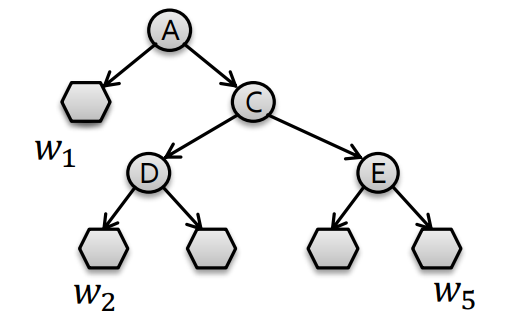
\includegraphics[width=0.45\textwidth]{images/decision-trees/decision-trees-17.png}
    \end{center}

    \item Define complexity of tree \( f \) as:
    \[
        \Omega(f) = \gamma \cdot T + \frac{1}{2} \lambda \sum_{j=1}^{T} w_j^2
    \]
    where:
    \begin{itemize}
        \item \( T \): number of leaves of tree \( f \)
        \item \( \gamma \): cost of adding a leaf to the tree \( f \)
    \end{itemize}
\end{itemize}
\end{frame}


\begin{frame}{Revisiting the Objective}
\begin{itemize}
    \item \textbf{Define:}
    \begin{itemize}
        \item The set of examples in the leaf \( j \):
        \[
            I_j = \left\{ i \mid q(x_i) = j \right\}
        \]
        where \( q(x) \) denotes the leaf that data point \( x \) belongs to.
    \end{itemize}

    \item The parameters that depend on the loss:
    \[
        G_j = \sum_{i \in I_j} g_i \qquad H_j = \sum_{i \in I_j} h_i
    \]

    \item Then the objective function becomes:
    \[
        \text{obj}^{(t)} = \sum_{j=1}^{T} \left[ G_j w_j + \frac{1}{2}(H_j + \lambda) w_j^2 \right] + \gamma T
    \]
\end{itemize}
\end{frame}


\begin{frame}{How to find a single tree \( f_t \)}
\begin{itemize}
\item Given a tree \( f_t \), we know how to
\begin{itemize}
    \item Calculate the score for \( f \):
    \[
        \text{Obj} = -\frac{1}{2} \sum_{j=1}^{T} \frac{G_j^2}{H_j + \lambda} + \gamma T
    \]

    \item And then set optimal weights for the chosen \( f \):
    \[
        w_j^* = -\frac{G_j}{H_j + \lambda}
    \]
\end{itemize}


\item In principle we could:
\begin{itemize}
    \item Enumerate possible tree structures \( f \) and take the one that minimizes \( \text{Obj} \)
\end{itemize}
\end{itemize}
\end{frame}

\begin{frame}{How to find a single tree \( f_t \)}
\begin{itemize}
\item In practice we grow tree greedily:
\begin{itemize}
    \item Start with tree with depth 0
    \item For each leaf node in the tree, try to add a split
    \item The change of the objective after adding a split is:
\end{itemize}

\[
\text{Gain} = \frac{1}{2} \left[ \frac{G_L^2}{H_L + \lambda} + \frac{G_R^2}{H_R + \lambda} - \frac{(G_L + G_R)^2}{H_L + H_R + \lambda} \right] - \gamma
\]

\begin{itemize}
    \item Take the split that gives best gain
\end{itemize}

\item Next: \textbf{How to find the best split?}
\end{itemize}
\end{frame}


\begin{frame}{How to Find the Best Split?}

\begin{itemize}
    \item For each node, enumerate over all features:
    \begin{itemize}
        \item For each feature, sort the instances by feature value
        \item Use a linear scan to decide the best split along that feature
        \item Take the best split solution along all the features
    \end{itemize}
    
    \item Pre-stopping:
    \begin{itemize}
        \item Stop split if the best split has negative gain
        \item But maybe a split can benefit future splits
    \end{itemize}
    
    \item Post-pruning:
    \begin{itemize}
        \item Grow a tree to maximum depth, recursively prune all the leaf splits with negative gain
    \end{itemize}
\end{itemize}

\end{frame}

\begin{frame}{Summary: GBDT Algorithm}

\begin{itemize}
    \item Add a new tree $f_t(x)$ in each iteration
    \begin{itemize}
        \item Compute necessary statistics for our objective
        \[
            g_i = \partial_{\hat{y}^{(t-1)}} l(y_i, \hat{y}^{(t-1)}), \quad
            h_i = \partial^2_{\hat{y}^{(t-1)}} l(y_i, \hat{y}^{(t-1)})
        \]
        \item Greedily grow the tree that minimizes the objective:
        \[
            Obj = -\frac{1}{2} \sum_{j=1}^{T} \frac{G_j^2}{H_j + \lambda} + \gamma T
        \]
    \end{itemize}
    
    \item Add $f_t(x)$ to our ensemble model
    \[
        y^{(t)} = y^{(t-1)} + \epsilon f_t(x_i)
    \]
    $\epsilon$ is called step-size or shrinkage, usually set around 0.1.  
    Goal: prevent overfitting.

    \item Repeat until we use $M$ ensemble of trees
\end{itemize}

\end{frame}


\begin{frame}{XGBoost}

\begin{itemize}
    \item \textbf{XGBoost}: \textbf{eXtreme Gradient Boosting}
    \begin{itemize}
        \item A highly scalable implementation of gradient boosted decision trees with regularization
    \end{itemize}

    \item Widely used by data scientists and provides state-of-the-art results on many problems!

    \item System optimizations:
    \begin{itemize}
        \item Parallel tree constructions using column block structure
        \item Distributed Computing for training very large models using a cluster of machines.
        \item Out-of-Core Computing for very large datasets that don’t fit into memory.
    \end{itemize}
\end{itemize}

\end{frame}
